\documentclass[letterpaper]{scrartcl}

\usepackage[nochapters]{classicthesis}
\usepackage[TextAligned,NoDate]{currvita}
\usepackage{hyperref,fullpage,xcolor,graphicx}

\renewcommand{\cvheadingfont}{\Huge}
\renewcommand{\cvlistheadingfont}{\textbf\large}
\hypersetup{colorlinks,breaklinks,urlcolor=cyan,linkcolor=cyan}

\begin{document}
\begin{cv}{Luis Alejandro Mart\'inez Faneyth}
\vspace{1em}

\begin{minipage}[ht]{.7\linewidth}
\begin{cvlist}{Datos Personales}
\item[\textit{\small{nacimiento}}]{Caracas, Venezuela --- 26 de Julio de 1986}
\item[\textit{\small{email}}]{\href{mailto:luis@huntingbears.com.ve}{luis@huntingbears.com.ve}}
\item[\textit{\small{blog}}]{\href{http://huntingbears.com.ve/}{huntingbears.com.ve}}
\item[\textit{\small{gitorious}}]{\href{http://gitorious.org/~huntingbears}{gitorious.org/$\sim$huntingbears}}
\item[\textit{\small{github}}]{\href{http://github.com/HuntingBears}{github.com/HuntingBears}}
\end{cvlist}
\end{minipage}
\begin{minipage}[ht]{.3\linewidth}
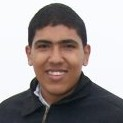
\includegraphics{huntingbears.jpg}
\end{minipage}
\vspace{1em}

\begin{cvlist}{Formaci\'on acad\'emica}
\item[{\parbox[t]{6em}{\textit{\large{2009}}}}]{
	\parbox[t]{\linewidth}{
		\textbf{Universidad Nacional Experimental de la Fuerza Armada} --- Maracay, Venezuela\\
		\textit{Ingeniero de Telecomunicaciones}
	}
}
\end{cvlist}
\vspace{1em}

\begin{cvlist}{Cursos de actualizaci\'on}
\item[{\parbox[t]{6em}{\textit{\large{2011}}}}]{
	\parbox[t]{\linewidth}{
		\textbf{Centro Nacional de Adistramiemto} --- Caracas, Venezuela\\
		\textit{Administraci\'on del tiempo y productividad laboral} --- 16 Horas\\
		\footnotesize{T\'ecnicas organizativas, trabajo en equipo, cooperaci\'on y complementariedad, establecimiento de prioridades, cronogramas de actividades, valoraci\'on del tiempo.}
	}
}
\item[{\parbox[t]{6em}{\textit{\large{2011}}}}]{
	\parbox[t]{\linewidth}{
		\textbf{Centro Nacional de Tecnolog\'ias de la Informaci\'on} --- Caracas, Venezuela\\
		\textit{Python avanzado} --- 32 Horas\\
		\footnotesize{Estructuras, entornos virtuales, versionamiento (Mercurial, Git), reStructured Text, documentaci\'on con sphinx, plataformas web, django, bases de datos (Sqlite), GUI (pyGTK, pyQT), iteradores, generadores, decoradores, pruebas unitarias.}
	}
}
\item[{\parbox[t]{6em}{\textit{\large{2011}}}}]{
	\parbox[t]{\linewidth}{
		\textbf{Centro Nacional de Tecnolog\'ias de la Informaci\'on} --- Caracas, Venezuela\\
		\textit{Python b\'asico} --- 16 Horas\\
		\footnotesize{Int\'erprete, l\'inea de comandos, librer\'ia est\'andar, funciones b\'asicas, tipos de datos, m\'odulos, estructuras, ciclos, interacci\'on con el usuario y el sistema operativo, operaciones aritm\'eticas, formato de resultados, tratamiento de errores.}
	}
}
\item[{\parbox[t]{6em}{\textit{\large{2011}}}}]{
	\parbox[t]{\linewidth}{
		\textbf{Fundaci\'on Hoatzin} --- Caracas, Venezuela\\
		\textit{Administraci\'on de sitios en Plone con Cyn.in} --- 40 Horas\\
		\footnotesize{Instalaci\'on de Plone con Unified Installer y zc.buildout. Configuración, apariencia, roles de usuario, instalaci\'on de productos, Zope y ZODB.}
	}
}
\end{cvlist}
\vspace{1em}

\begin{cvlist}{Eventos (ponente)}
\item[{\parbox[t]{6em}{\textit{\large{2010}}}}]{
	\parbox[t]{\linewidth}{
		\textbf{3ra Cayapa Canaima} --- Barquisimeto, Venezuela\\
		\textit{Eficiencia de contenidos con PHP}
	}
}
\item[{\parbox[t]{6em}{\textit{\large{2011}}}}]{
	\parbox[t]{\linewidth}{
		\textbf{7mo Congreso Nacional de Software Libre} --- Barquisimeto, Venezuela\\
		\textit{Canaima 3.0: ¿Qu\'e hay de nuevo?}
	}
}
\item[{\parbox[t]{6em}{\textit{\large{2011}}}}]{
	\parbox[t]{\linewidth}{
		\textbf{Festival Latinoamericano de Instalaci\'on de Software Libre} --- M\'erida, Venezuela\\
		\textit{Canaima 3.0: ¿Qu\'e hay de nuevo?}
	}
}
\item[{\parbox[t]{6em}{\textit{\large{2011}}}}]{
	\parbox[t]{\linewidth}{
		\textbf{7mo D\'ia Debian} --- Caracas, Venezuela\\
		\textit{Haciendo distribuciones derivadas con Canaima Semilla}
	}
}
\item[{\parbox[t]{6em}{\textit{\large{2011}}}}]{
	\parbox[t]{\linewidth}{
		\textbf{Tecnolog\'ias de Informaci\'on Libres para Vivir Viviendo} --- Caracas, Venezuela\\
		\textit{¿Como hacer un sabor de Canaima?}
	}
}
\item[{\parbox[t]{6em}{\textit{\large{2012}}}}]{
	\parbox[t]{\linewidth}{
		\textbf{Festival Latinoamericano de Instalaci\'on de Software Libre} --- Maracaibo, Venezuela\\
		\textit{¿C\'omo desarrollar para Canaima GNU/Linux}
	}
}
\item[{\parbox[t]{6em}{\textit{\large{2012}}}}]{
	\parbox[t]{\linewidth}{
		\textbf{Conferencia de Desarrolladores de Debian (DebConf)} --- Managua, Nicaragua\\
		\textit{Haciendo distribuciones derivadas con Canaima Semilla}
	}
}
\end{cvlist}
\vspace{1em}

\begin{cvlist}{Eventos (asistente)}
\item[{\parbox[t]{6em}{\textit{\large{2007}}}}]{
	\parbox[t]{\linewidth}{
		\textbf{Simposio Internacional de Telecomunicaciones} --- M\'erida, Venezuela\\
	}
}
\item[{\parbox[t]{6em}{\textit{\large{2011}}}}]{
	\parbox[t]{\linewidth}{
		\textbf{7mo Congreso Nacional de Software Libre} --- Caracas, Venezuela\\
	}
}
\end{cvlist}
\vspace{1em}

\begin{cvlist}{Experiencia laboral}
\item[{\parbox[t]{6em}{\textit{\large{Nov 2009\\Actual}}}}]{
	\parbox[t]{\linewidth}{
		\textbf{Centro Nacional de Tecnolog\'ias de Informaci\'on} --- Caracas, Venezuela\\
		\textit{Administrador de Plataforma Tecnol\'ogica}\\
		\footnotesize{Desarrollo del Sistema Operativo Canaima GNU/Linux. Dise\~no e implementaci\'on de soluciones inform\'aticas en Software Libre. Administraci\'on de Servicios. Soporte de alto nivel.}
	}
}
\item[{\parbox[t]{6em}{\textit{\large{Oct 2010\\Abr 2011}}}}]{
	\parbox[t]{\linewidth}{
		\textbf{Universidad Nacional Experimental de la Fuerza Armada} --- Maracay, Venezuela\\
		\textit{Docente}\\
		\footnotesize{Ense\~nanza de los sistemas de numeraci\'on, operaciones aritm\'eticas, representaci\'on de sistemas digitales, compuertas l\'ogicas, sistemas s\'incronos y as\'incronos, flip-flops, memorias.}
	}
}
\item[{\parbox[t]{6em}{\textit{\large{Nov 2008\\Nov 2009}}}}]{
	\parbox[t]{\linewidth}{
		\textbf{NETUNO, C.A.} --- Maracay, Venezuela\\
		\textit{T\'ecnico de Levantamiento}\\
		\footnotesize{Dise\~no de Proyectos para la creaci\'on y ampliaci\'on de Redes Coaxiales para voz, datos y TV bajo el est\'andar DOCSIS. Supervisi\'on de la construcci\'on de Redes H\'ibridas. Levantamiento de informaci\'on en sitio. Diagramaci\'on con Autocad. Gesti\'on de Materiales y Supervisi\'on de Contratistas.}
	}
}
\item[{\parbox[t]{6em}{\textit{\large{May 2008\\Nov 2009}}}}]{
	\parbox[t]{\linewidth}{
		\textbf{Freelance} --- Maracay, Venezuela\\
		\textit{Docente}\\
		\footnotesize{Ense\~nanza de maquetamiento de p\'aginas web a trav\'es de HTML y CSS, usando tecnolog\'ias libres. Agregando interactividad con javascript (jQuery). P\'aginas din\'amicas con PHP. Creaci\'on y consulta de bases de datos basadas en SQL. Animaci\'on de secuencias con Adobe Flash. ActionScript.}
	}
}
\end{cvlist}

\begin{cvlist}{Publicaciones periodísticas}
\item[{\parbox[t]{6em}{\textit{\large{Mayo 2011}}}}]{
	\parbox[t]{\linewidth}{
		\textbf{Emisora de radio Alba Ciudad 96.3FM} --- Caracas, Venezuela\\
		\textit{Copiate esta Radio} --- Lanzamiento de Canaima 3.0
	}
}
\item[{\parbox[t]{6em}{\textit{\large{Mayo 2011}}}}]{
	\parbox[t]{\linewidth}{
		\textbf{Emisora de radio RNV Activa 103.9FM} --- Caracas, Venezuela\\
		\textit{Trinchera Digital} --- Lanzamiento de Canaima 3.0
	}
}
\item[{\parbox[t]{6em}{\textit{\large{Mayo 2011}}}}]{
	\parbox[t]{\linewidth}{
		\textbf{Venezolana de Televisi\'on} --- Caracas, Venezuela\\
		\textit{Rueda de Prensa MCTI} --- Lanzamiento de Canaima 3.0
	}
}
\end{cvlist}
\vspace{1em}

\begin{cvlist}{Reconocimientos}
\item[{\parbox[t]{6em}{\textit{\large{2012}}}}]{
	\parbox[t]{\linewidth}{
		\textbf{Centro Nacional de Tecnolog\'ias de la Informaci\'on} --- Caracas, Venezuela\\
		\textit{Desempe\~no excepcional}
	}
}
\end{cvlist}
\vspace{1em}

\begin{cvlist}{Habilidades}
\item[\textit{\large{Idiomas}}]{
	Espa\~nol --- Lectura/Escritura/Conversacional: Avanzado.\\
	Ingl\'es--- Lectura/Escritura/Conversacional: Avanzado.
}
\item[\textit{\large{Sistemas}}]{Manejo de ambientes GNU/Linux, Windows y MacOS.}
\item[\textit{\large{Programaci\'on}}]{C, C++, Python, Perl, PHP, Shell script, Make, AWK, Javascript.}
\item[\textit{\large{Bases de Datos}}]{Postgres, MySQL, SQL.}
\item[\textit{\large{Diagramaci\'on}}]{XML, HTML (4.x -- 5), reStructuredText, \LaTeX\, CSS.}
\item[\textit{\large{Dise\~no}}]{GIMP, Inkscape, Adobe Photoshop.}
\item[\textit{\large{Otros}}]{
	Generaci\'on de paquetes de software bajo las pol\'iticas de Debian.\\
	Generaci\'on de im\'agenes instalables a partir de distribuciones derivadas de Debian.
}
\end{cvlist}

\end{cv}
\end{document}
